\begin{figure}[h]
  \begin{center}
      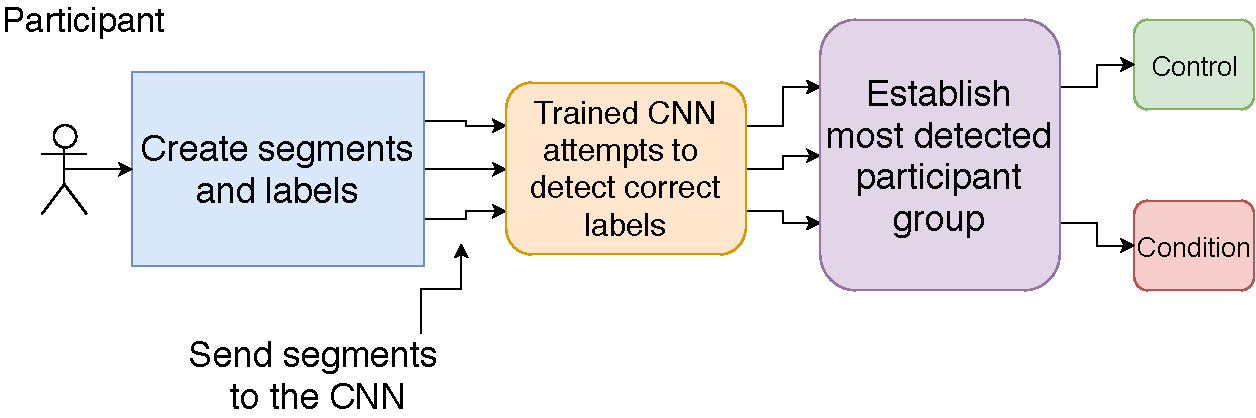
\includegraphics[height=4cm]{img/flow_detection.pdf}
      \caption{Diagram of how we detect whether a participant most likely belongs to the control or condition group (first objective) after we have trained the neural network. }
      \label{figure:flow}
  \end{center}
\end{figure}

As described in chapter \ref{chapter:introduction}, our objectives in this thesis are creating convolutional neural network models for three different tasks:

\begin{itemize}
  \item Detect whether a participant belongs to the \textbf{control} group or \textbf{condition} group.
  \item Detect a participant's depression level (by MADRS score).
  \item Predict a participant's MADRS score.
\end{itemize}

The input data to our neural networks is time-sliced segments of motor activity measurements. We send the segments to the neural networks, which attempts to detect the correct value for each segment. During the training process, correct values have to be visible to the model for it to learn (because we use a supervised learning strategy). After training the models, they should be able to classify/predict the correct value depending on the objective. Because we split the measurements of a participant into segments, we needed to gather all of the detected value so that we could return one final detection. Majority voting is the method used for this, which means that we use the most popular detection (label with most \textit{votes}). 

We implemented one-dimensional convolutional neural networks that were able to take the segments of activity data as input. Also, we wanted the neural network models to be as similar as possible. With few changes in the layers (preferably only the last few layers), we could use a model on another objective. It was, however, only possible for the first two objectives, as they are both about classification and we only changed the number of units in the output layer. We changed more layers for the third objective. We describe of all neural network models in detail in chapter \ref{chapter:models}.

In this chapter, we describe the structure of the dataset, how we use the dataset to create activity segments, and how we can test and evaluate the performance of machine learning models.

\section{The dataset}

\begin{figure}[h]
  \begin{center}
      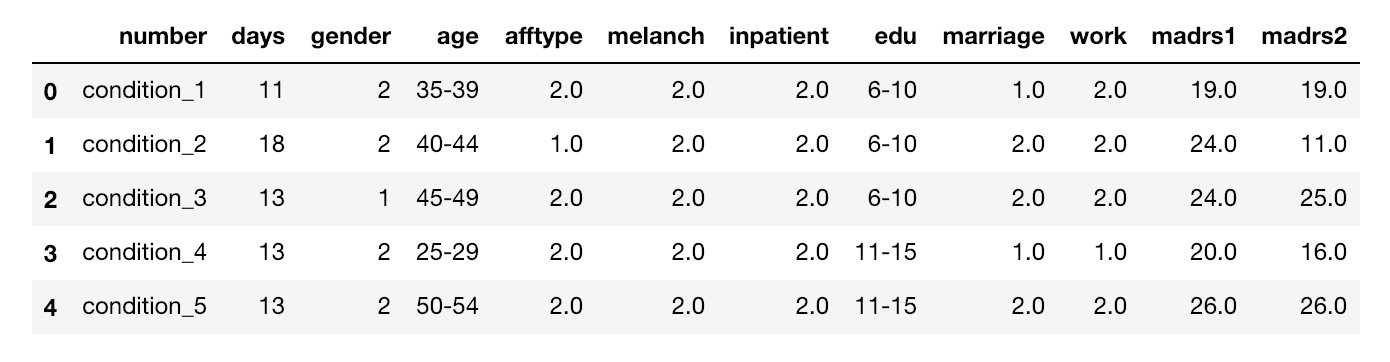
\includegraphics[height=3.5cm]{img/demographics.png}
      \caption{The 5 first rows in demographic dataset (scores.csv). The displayed participants are from the condition group.}
      \label{figure:demographics}
  \end{center}
\end{figure}

\begin{figure}[h]
  \begin{center}
      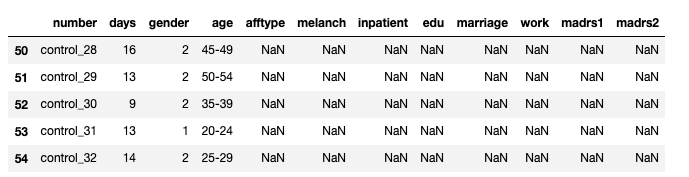
\includegraphics[height=3.5cm]{img/demographics_control.png}
      \caption{The 5 last rows in demographic dataset (scores.csv). The displayed participants are from the control group.}
      \label{figure:demographics_control}
  \end{center}
\end{figure}

\begin{figure}[h]
  \begin{center}
      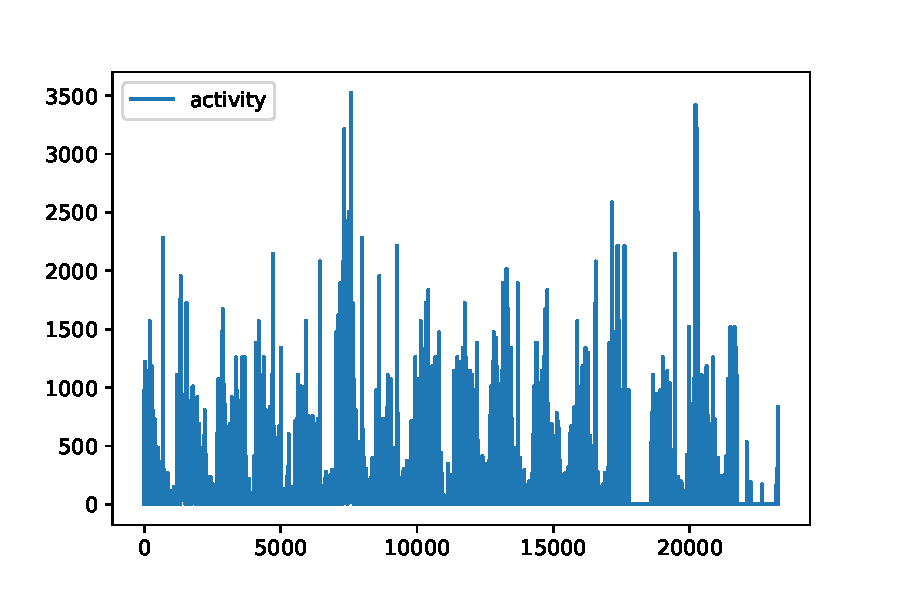
\includegraphics[height=7cm]{img/activity_condition_1.pdf}
      \caption{Motor activity measurements for a participant in the condition group. The participant is a male between 39 and 39 years old, diagnosed with unipolar depression. The number on the X-axis corresponds to the minute throughout the measurement period, and the number on the Y-axis is the activity levels.}
      \label{figure:participant_activity}
  \end{center}
\end{figure}

\begin{figure}[h]
  \begin{center}
    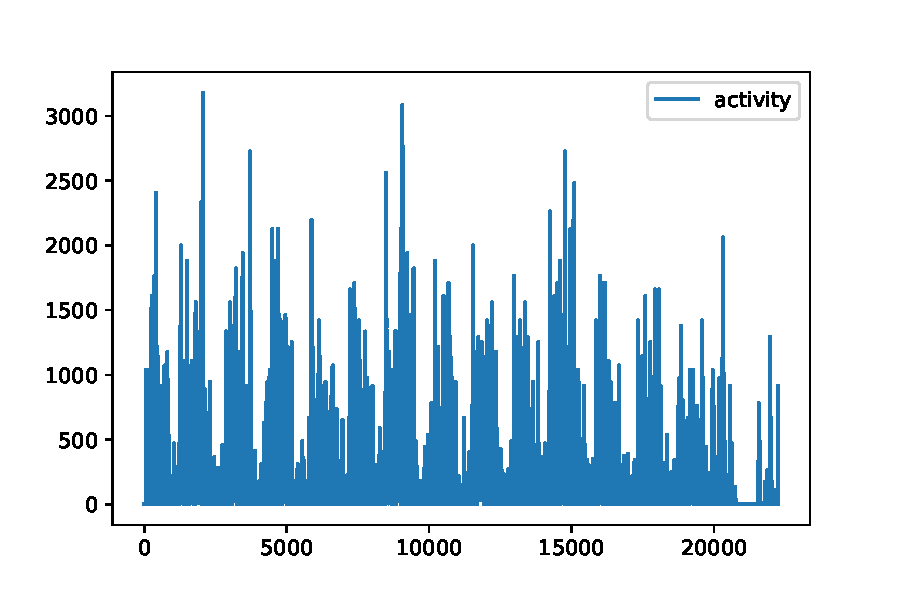
\includegraphics[height=7cm]{img/activity_control_1.pdf}
    \caption{Motor activity measurements for a participant in the control group. The participant is a female between 45 and 49 years old. The number on the X-axis corresponds to the minute throughout the measurement period, and the number on the Y-axis is the activity levels.}
    \label{figure:participant_activity_control}
  \end{center}
\end{figure}

In this thesis, we used a dataset containing motor activity measurements from participants wearing an Actiwatch (model AW4 from Cambridge Neurotechnology Ltd, England). The dataset was collected originally for a study about behavioral patterns in schizophrenia vs. major depression \cite{Berle2010}. The participants we focus on are 23 bipolar/unipolar patients and 32 non-depressed contributors, removing the participants with schizophrenia. From now on, we will refer to the bipolar/unipolar group as the \textit{condition group}, and the non-depressed group as the \textit{control group}. Garcia-Ceja et al. also follows this convention in their work \cite{GarciaCeja2018_classification_bipolar}.

The dataset is in two parts. One part includes the demographics of each participant (see figure \ref{figure:demographics}), where the fields are:

\begin{itemize}
    \item \textbf{number}: a unique id for each participant
    \item \textbf{days}: number of days of data collection 
    \item \textbf{gender}: 1 = female and 2 = male
    \item \textbf{age}: age of the participant (grouped by four years)
    \item \textbf{afftype}: affliction type, where 1 is for bipolar type II, 2 equals unipolar depressive, and 3 for participants with bipolar type I
    \item \textbf{melanch}: 1 means a participant has melancholia, 2 means no melancholia
    \item \textbf{inpatient}: whether the patient is inpatient (1) or outpatient (2)
    \item \textbf{edu}: how many years of education the participant has completed (grouped by four years)
    \item \textbf{marriage}: married/cohabiting (1) or single (2)
    \item \textbf{work}: whether the participant is working/studying (1) or not (2)
    \item \textbf{madrs1}: MADRS score before activity measurement started
    \item \textbf{madrs2}: MADRS score after activity measurements ended
\end{itemize}

The second part of the dataset includes motor activity measurements about participants in the condition group and control group, as one file for each participant. These files are placed in two folders for the two groups respectively, and there is one file for each participant with filename as "GROUP\_X.csv" where X is their id and GROUP is either condition or control. Inside each file, we can find a list of motor activity measurements for every minute of the data collection period.

Looking at example participants from both groups (figures \ref{figure:participant_activity} and \ref{figure:participant_activity_control}), we can not immediately tell that they are different with our eyes. However, by feeding the data into a convolutional neural network, we aimed to find patterns that were specific to the two groups. 

\section{Data Preprocessing}
\label{section:data_preprocessing}

We wrote a function \textit{create\_segments\_and\_labels()} (source code \ref{code:reading_dataset}), which was responsible of creating the data that is sent into the neural network. We started by defining a \textit{segment length} ($L$), which is how much data (minutes) we want inside each segment. We experiment with the value of $L$ in chapter \ref{chapter:training}. Next, we needed a value for how many indexes to step after each iteration, $S$. We kept this value at one hour, meaning $S=60$. Between the different objectives, this function will only be different in how it yields the \textit{labels}.

\begin{itemize}
  \item First we read the \textit{global} dataset, where we find each participant and whether they are in the control or condition group. As there is no \textit{afftype} value for non-depressed participants, we set this to 0. Other possible values are 1, 2 and 3. We do the same for the \textit{madrs2} column.
  \item Then we iterate over the participants:

  \begin{itemize}
    \item Build segments and labels arrays for current participant:
    \begin{itemize}
      \item Append a \textbf{segment} that is of length $L$ to the list of segments. 
      \item Append a value to labels depending on the objective (see the subsection about output data).
      \item Increase the index by $S$, then repeat until we have added all segments for the current participant.
    \end{itemize}
    \item Example element in segments and labels for a participant in the condition group: \\
    \textbf{segments[i] = [[0], [143], [0], [20], [166], [160], [306], [277]]}\\
    \textbf{labels[i] = [[1], [1], [1], [1], [1], [1], [1], [1]]}
  \end{itemize}
  
  \item Make the list of labels into a \textit{categorical} 2D matrix (see table \ref{table:categorical_labels}) with a \textbf{1} in only one of the columns, instead of a single-dimensional list. This is only needed in the first two objectives.
\end{itemize}

\subsection{Output data}

\begin{table}[h]
  \begin{center}
    \begin{tabular}{| l | l |}
      \hline
      \textbf{Control group} & \textbf{Condition group}  \\ \hline
      0                    &  1                \\ \hline
      1                    &  0                \\ \hline
      0                    &  1                \\ \hline
      1                    &  0                \\ \hline
      1                    &  0                \\ \hline
      0                    &  1                \\ \hline
      0                    &  1                \\ \hline
      1                    &  0                \\ \hline
    \end{tabular}
    \caption{Categorical Labels. A 0 and a 1 (first row) means that the participant is in the condition group.}
    \label{table:categorical_labels}
  \end{center}
\end{table}

The output data was an array with a value for each segment, corresponding to the objective and the participant. After creating it, we used a helper function from Keras called \textit{to\_categorical} to transform the array into a categorical matrix instead of a list of labels. Table \ref{table:categorical_labels} is an example of how a categorical matrix looks. The value we used to build this array was based on the objective:

\begin{itemize}
  \item For classifying control/condition group, this list was built to contain the values \textbf{0} or \textbf{1} for the labels \textbf{CONTROL} and \textbf{CONDITION}, which was chosen according to the group the participants were in. For example, \textbf{labels[i] = [0, 1]}, meaning that segment $i$ is labeled as \textbf{CONDITION} group. 
  
  \item To classify depression classes, we used MADRS scores divided into four classes by some cutoff-points:
  \begin{itemize}
    \item 0-6: normal
    \item 7-19: mild depression
    \item 20-34: moderate depression
    \item 34-60: severe depression
  \end{itemize}
  So instead of labelling the segments as \textbf{CONTROL} or \textbf{CONDITION}, we labeled them as \textbf{NORMAL}, \textbf{MILD} and \textbf{MODERATE} (we ignored severe depression as there are no participants with MADRS scores this high). An example element in this array after applying \textit{to\_categorical()} is \textbf{labels[i] = [0, 1, 0]}, which means that segment $i$ is labeled as \textbf{MILD} depression.
  \item For predicting MADRS scores, we built the array of the MADRS score of the participants. Example: \textbf{scores[i] = [18]}.
\end{itemize}

\section{Performance}

When finishing with a training session for a machine learning model, we need to use different metrics to be able to tell how the model performed based on some testing data. For prediction models, we only consider the value returned by the \textit{loss function}, but evaluation of classification models can be presented with several metrics. In this section we present loss functions and optimizers, and how we evaluate the performance of our models using classification metrics and different ways of splitting up into training and testing data.

\subsection{Loss functions and Optimizers}

After defining a machine learning model, we \textit{compile} it so that it was ready to be \textit{fit} to the dataset. Compiling a model requires a \textit{loss function} and an \textit{optimizer}. The loss function is the function that evaluates how well the model \textit{models} the given data \cite{loss_functions}, and the optimizer is the function that attempts to lower the output of the loss function. 

For the first two objectives in this thesis, we use the loss function \textit{categorical crossentropy}, which calculates a probability over the number of classes supplied (number of classes equals the number of neurons in the output layer) \cite{cross_entropy}. In the third objective, we use a loss function called \textit{Mean Squared Error (MSE)}, which is measured as the average (mean) of squared difference between predictions and actual observations \cite{loss_functions}. 
\[ MSE = \frac{\sum_{i=1}^{n}(y_i-\hat{y}_i)^2}{n} \]

When choosing an optimizer, there are many different options available, but we chose an optimizer called \textit{Adam} for training all of our models. Adam is an algorithm for efficient stochastic gradient-based optimization \cite{adam}, and it is available as an optimizer function within the Keras framework \cite{keras_docs}. The reason for choosing Adam is, as described by Kingma, D. P. et al. \cite{adam}, efficient both considering memory usage and computationally. The hyper-parameters also require minimal tuning. Using a different optimizer can make the model fit the dataset at a different pace, which is something we experiment with in chapter \ref{chapter:training} (for the third objective). 

\subsection{Classification metrics}
In classification, accuracy is a metric that is commonly used. It makes sense to the human brain; telling a friend that has no experience in machine learning or data science that we have made our computer able to classify something with 98\% accuracy is something that they would understand. Other metrics include \textit{precision}, \textit{recall}, \textit{specificity} and \textit{F1 score} \cite{GarciaCeja2018_classification_bipolar}, which will be described below.

\subsubsection{Confusion matrix}

\begin{figure}[h]
  \begin{center}
    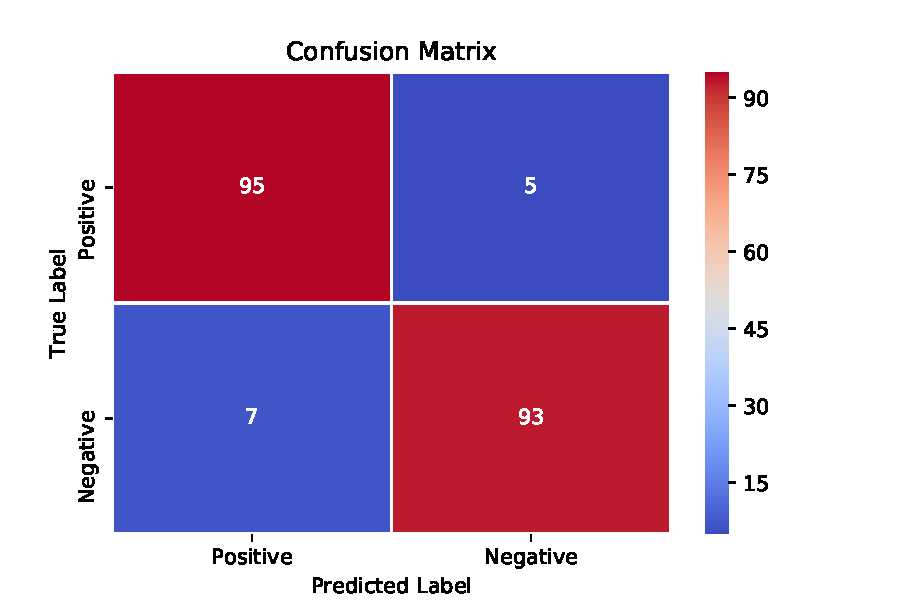
\includegraphics[height=8cm]{img/conf_matrix.pdf}
    \caption{Confusion Matrix Example: 95 True Positives, 93 True Negatives, 7 False Positives and 5 False Negatives}
    \label{figure:confusion_matrix_bipolar}
  \end{center}
\end{figure}

Figure \ref{figure:confusion_matrix_bipolar} shows a \textit{confusion matrix}. It is a visual metric for classification models in machine learning and is the basis for the other performance metrics. It can tell how well our model is performing by having correlation values for the different classes. Let us say we have 200 samples in our test data to use on our model that classifies control vs. condition group. 

A \textit{confusion matrix} for a good model would look like figure \ref{figure:confusion_matrix_bipolar}, with high numbers in \textbf{True Positive} and \textbf{True Negative} and as low numbers as possible in \textbf{False Positive} and \textbf{False Negative}. Having a high number in \textbf{True Positive} means that the model can classify that a participant is in the condition group if he or she is, and having a high number in \textbf{True Negative} means that the model can classify that a participant is in the control group if this is the case. The other cases, \textbf{False Positive} and \textbf{False Negative}, is where the model made a wrong classification, and therefore as close these numbers are to zero the better our model is.

\subsubsection{Accuracy}

\blockquote[\cite{ml_metrics}]{Accuracy is a good measure when the target variable classes in the data are nearly balanced.}

When calculating the \textit{accuracy}, we sum up the correct predictions and divide that with the total number of predictions ($ \frac{TP + TN}{TP + TN + FN + FP} $). For our example (\ref{figure:confusion_matrix_bipolar}), the \textit{accuracy} would be $ \frac{93 + 95}{93 + 95 + 5 + 7} = 0.94 $. It is a good metric to use for our example because the number of samples for each variable class is well balanced ($ 93+5=98 $ samples where \textbf{condition group} was the correct option, and $ 7+95=102 $ samples where \textbf{control group} was correct).

Terrible use of the \textit{accuracy} metric would be when one of the classes strongly dominates the samples. For example, if a model predicts \textbf{cancer} vs. \textbf{no cancer}, and the samples contain five people with cancer, and the 95 remaining people do not. The model would be terrible at predicting cancer and still have an accuracy score of $ 0.95 $ \cite{ml_metrics}.

\subsubsection{Precision} 

Precision operates entirely on the predicted positives, and it tells us how many \textbf{true positives} there is among \textbf{predicted positives} ($ \frac{TP}{TP + FP} $) \cite{ml_metrics}. 

This performance metric is better to use on \textit{unbalanced} classes than accuracy. The \textit{cancer vs no cancer} example, assuming it predicts no-one to have \textbf{cancer}, would yield a precision score of $ \frac{5}{5+95} = 0.05 $. And our \textit{control vs condition} example would result in a precision score of $ \frac{93}{93+7} = 0.93 $.

\subsubsection{Recall}

\textit{Recall} is another useful performance metric. It tells us the relationship between \textbf{true positives} and \textbf{actual positives}, for example how many participants classified to be in the condition group there were among total participants in the condition group.

The calculation of recall is done by dividing \textbf{true positives} by \textbf{true positives + false negatives} ($ \frac{TP}{TP+FN} $), which translates into $ \frac{93}{93+5} \approx 0.95 $ (using the confusion matrix) \ref{figure:confusion_matrix_bipolar}.

Choosing a metric to use from \textit{precision} or \textit{recall} depends on your goal. Try to achieve close to $ 1.0 $ \textit{recall} if you want to reduce \textbf{false negatives}, and likewise with \textit{precision} if you want to reduce \textbf{false positives} \cite{ml_metrics}.

\subsubsection{Specificity}

As \textit{recall} operates on \textbf{actual positives}, \textit{specificity} is the exact opposite metric. It tells us the relationship between \textbf{true negatives} and \textbf{actual negatives}. So if your goal is to reduce \textbf{false positives}, specificity is a valid choice. \textit{Specificity} is calculated by dividing \textbf{true negatives} by \textbf{true negatives + false positives} ($ \frac{TN}{TN+FP} $). For the confusion matrix \ref{figure:confusion_matrix_bipolar}, the \textit{specificity} score equals $ \frac{95}{95+7} \approx 0.93 $.

\subsubsection{F1 Score}

The metrics that we have described in this section are all useful when determining whether our classification model is good enough. However, the relationship between \textit{recall} and \textit{precision} and knowing when to use which can be confusing, at least if the different classes are somewhere between entirely unbalanced and perfectly balanced (for example a 35\% split). 

Therefore another metric called \textit{F1 Score} was created, which gives us a balanced value combining \textit{recall (R)} and \textit{precision (P)}. The basic idea is to return the \textit{mean} value of the two scores (F1 = $ \frac{P + R}{2} $), but that would not be balanced if one score is much lower than the other. F1 score actually uses something called \textit{harmonic mean} instead of the standard \textit{arithmetic mean}, and is calculated as $ 2 \cdot \frac{P \cdot R}{P + R} $ \cite{ml_metrics}. 
Following this formula, the F1 score for confusion matrix \ref{figure:confusion_matrix_bipolar} becomes:

\[
  F1 = 2 \cdot \frac{P \cdot R}{P + R} = 2 \cdot \frac{0,93 \cdot 0,95}{0,93 + 0,95} \approx 0.94
\]

\subsection{Training and testing data}
\begin{figure}
  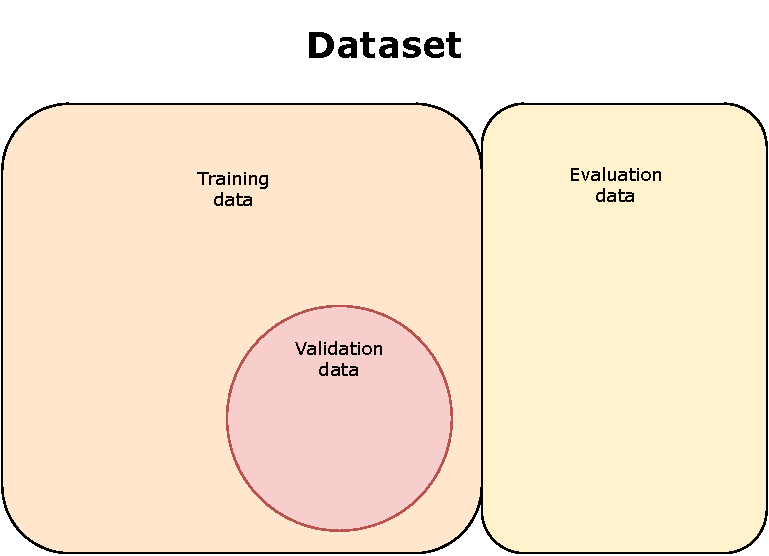
\includegraphics{img/train_test_data.pdf}
  \caption{Visualization of a dataset evaluation split. Training and evaluation data are subsets of the dataset, and the validation data is a subset of the training data.}
  \label{figure:dataset_train_test}
\end{figure}

It is common to split the inputs and output data into multiple parts, where some of the data is used to test the model. Testing of the model can happen at different times: after training sessions (evaluation) and in between epochs (validation). 

Before starting a model training session, we split the dataset into training and evaluation data, where the first part is what the model is trained to fit, and evaluation data is kept aside until the training is complete. Then we use it to check the performance of the trained model. Metrics used here is the value of the loss function (for example mean squared error) for value prediction, or classification metrics described above.

Validation data and is useful to include when we are developing the model, as we regularly see how the model is performing after each epoch. The metric used is usually the value of the loss function or the accuracy score, depending on the objective of the model. When the model is good enough for the desired task, we do not need validation data. We pass the validation split into the function that starts the model's training as either the validation\_split or the validation\_data parameter. If the validation\_split parameter is used (a number between 0 and 1), the validation data is calculated automatically before training starts. If, however, we want to use specific samples as validation data, we use the validation\_data parameter instead.

The function \textit{train\_test\_split} from the \textit{sklearn} package is useful to split up the dataset into training and evaluation data. We input dataset (X, y), plus how large we want the training and test sets to be (number between 0 and 1, which determines the size of the test partition). The function also randomizes the data, preventing model to accidentally learn something correct for segments in a row that also are chronologically in order. After calling the function, you end up with two arrays for input data (\textit{X\_train, X\_test}), and two arrays for output data (\textit{y\_train, y\_test}). In this case the \textit{test\_size} is set to $0.4$, meaning that the test set contains $40\%$ of the total dataset and the remaining $60\%$ are in the training set.

\begin{figure}[h]
\begin{code}
    \begin{minted}[linenos]{python}
from sklearn.model_selection import train_test_split

X_train, X_test, y_train, y_test = train_test_split(X, y, 
                                                    test_size=0.4)
    \end{minted}
    \caption{Sklearn train and test split. After calling this function we end up with training and testing sets for both inputs and outputs.}
    \label{code:sklearn_train_test_split}
\end{code}
\end{figure}

\begin{figure}[h]
  \begin{code}    
      \begin{minted}[linenos]{python}
      from sklearn.model_selection import StratifiedKFold
  
      X, y = load_data(...)
  
      skf = StratifiedKFold(n_splits=3, shuffle=True)
  
      for train_index, test_index in skf.split(X, y):
          X_train, X_test = X[train_index], X[test_index]
          y_train, y_test = y[train_index], y[test_index]
  
          model = create_model(...)
          model.fit(X_train, y_train, ...)
          results = model.evaluate(X_test, y_test)
  
          # do something with results...
  
      \end{minted}
      \caption{StratifiedKFold from sklearn. The dataset is split in 3 parts (n\_splits on line 5), then training and evaluation happens for each of the parts.}
      \label{code:sklearn_k_fold}
  \end{code}
\end{figure}
  

\subsubsection{Cross-validation}
Another popular choice is to use something called \textit{K-fold cross-validation}. It works by splitting the dataset into $K$ train and test sets, and for each of them, train the model on the training set and validate on the test set. Cross-validation is a good way of checking if your model's performance truly is independent on which data samples it trained on. The higher number of splits ($K$) means fewer data samples to test on, so you need to keep that in mind (the same for \textit{train\_test\_split} if you set the \textit{test\_size} too low). Sklearn has an implementation of \textit{K-fold}, called \textit{StratifiedKFold}. An example of how it can be used is shown in code \ref{code:sklearn_k_fold}, where we perform a 3-fold cross-validation ($K = 3$). 

Performance testing of a model sometimes happens with both train/test-split and cross-validation. We set aside a small part of the dataset for evaluation and generating folds for the rest, then within each fold, we train and validate the model, and evaluate it against the part of the dataset that we set aside at the beginning. We note loss/accuracy scores for each fold and calculate the mean value which is the overall performance result.

Another way of using cross-validation to test the performance of a model is by leaving N participants out of the dataset. We do this by generating training data for the rest of the participants and evaluation data for the N participants left out. We log the performance scores for each fold, and then we find the overall average. 

In this thesis, we will use all described methods of splitting training and testing data. Simple train/test splitting is what we begin with during the development of the models. Then we perform cross-validation to verify that the models are consistent, and finally, we leave participants out one by one. The latter is essentially the same as 55-fold cross-validation, and it is a way of comparing our work to the work of Garcia-Ceja, E. et al., where they also evaluated their models by leaving participants out one by one \cite{GarciaCeja2018_classification_bipolar}. 

\begin{figure}
\begin{center}
  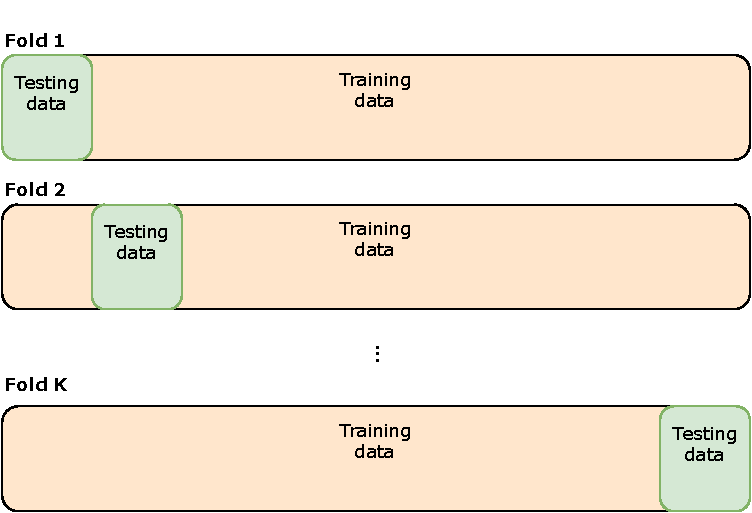
\includegraphics{img/Cross-validation.pdf}
  \caption{K-fold cross-validation visualized. For each fold, a testing set is defined, and the rest of the data is a training set.}
  \label{figure:dataset_cross_val}
\end{center}  
\end{figure}